% TODO
%
% - Explanation as to why multiplier increases with more flexible prices
% - Calculate the size of the multiplier out of the liquidity trap?


\section{The Government Spending Multiplier}

\subsection*{Definition of Government Spending Multiplier}

A key figure to decide whether a fiscal intervention by the government is desirable or not is the multiplier. We need to know (or at least estimate) what are the effects of a spending hike in the economy and the multiplier delivers important information about this question. The multiplier measures the impact that marginal variations of government spending has on output. It is defined as the increase in GDP generated by a marginal increase in government spending. If government steps in and spends one extra euro, it is not clear a priori how agents will react to that. It can be argued that this euro will be further spent by its recipient generating a virtuous circle that will ultimately boost the economy. On the other hand, spending increases also put pressure on government budget, which might trigger uncertainty about government's ability to pay its debt back. This in turn could lead agents to cut back on spending foreseeing hard times. In this case, an increase in government could trigger a fall on GDP.  In general lines, it is not clear what are the implications of government intervention in a crisis. Understanding the mechanism behind the multiplier and how it works can shed light on this question, because the multiplier is this one number that states whether an increase in government spending will ultimately boost or depress an economy and by how much. The multiplier $m_t$ can be expressed formally as
\begin{equation}
  m_t = \frac{dY_t}{dG_t} = \frac{1}{g_y}\frac{dy_t}{dg_t} \nonumber
\end{equation}
where capital letters stand for variables in levels and lowercase letters for variables expressed in deviations from steady state.

\subsection*{The Multiplier in the Model}

In the model, the multiplier has a stairway format. The multiplier is constant as long as the duration of the liquidity trap remains unchanged. This means that each extra euro spent by the government will have the same effect on output if the liquidity trap duration is not affected. Once the increase in government spending is big enough to shorten the duration of the liquidity trap by one period, the multiplier declines. Government spending becomes then less effective in boosting the economy.

\begin{figure}[th]
\centering
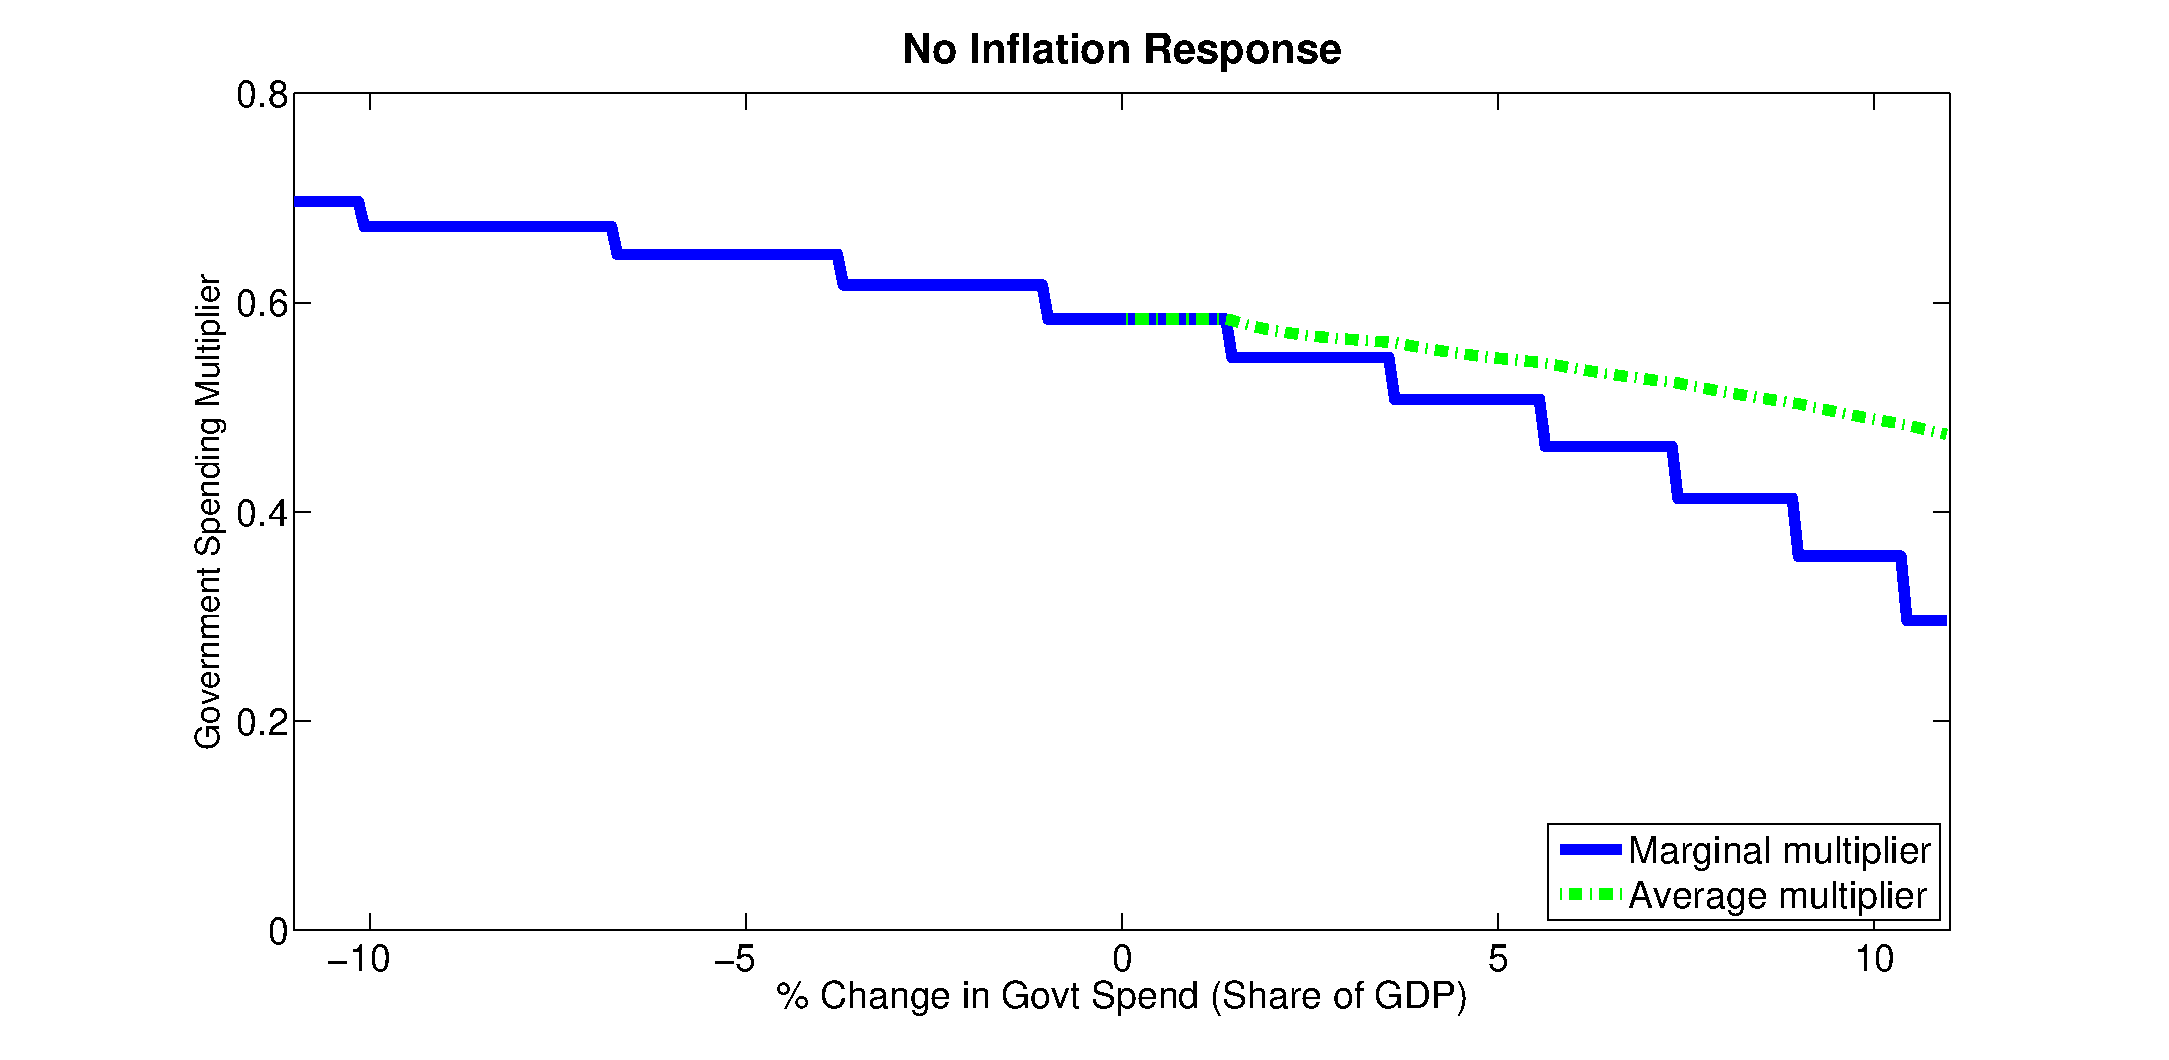
\includegraphics[width=0.8\textwidth]{paper/figures/figure-3-gsm-no-inflation}
\caption{Average and Marginal Spending Multiplier with No Inflation}
\label{fig:averagemultiplier}
\end{figure}

In Figure \ref{fig:averagemultiplier}, which depicts a model with no inflation, the multiplier is  0.584 by 0\% change in government spending. If policy makers decide to step in and increase spending, the multiplier remains constant at 0.584 until the increase in spending surpasses the threshold of 1.46\% of GDP. At this point, the liquidity trap becomes one period shorter, which makes the multiplier decrease to 0.548. This mechanism works in this fashion (big enough government spending hike leads to shorter liquidity trap and smaller multiplier) until the increase in government spending is so high that the economy gets out of the liquidity trap. After that, the multiplier is constant in the model irrespective of the size of the government in the economy.
The case we have been considering, in which prices do not vary at all, displays a relatively low multiplier. In fact, it is smaller than unity. Once we allow for the more realistic scenario with sticky but not completely fixed prices, the multiplier increases by a considerable amount. Figure \ref{fig:mulalt} shows the multiplier schedule for three different average price durations. The more flexible the prices, the higher the multiplier for a given level of government spending. With four-quarter contracts (Calvo parameter set to 0.75), the multiplier reaches a far greater value of 3.828. This means that each euro spent by the government will increase GDP by 3.828 euros (as long, of course, as the spending hike is not too big to shorten the liquidity trap).

\begin{figure}[!th]
\centering
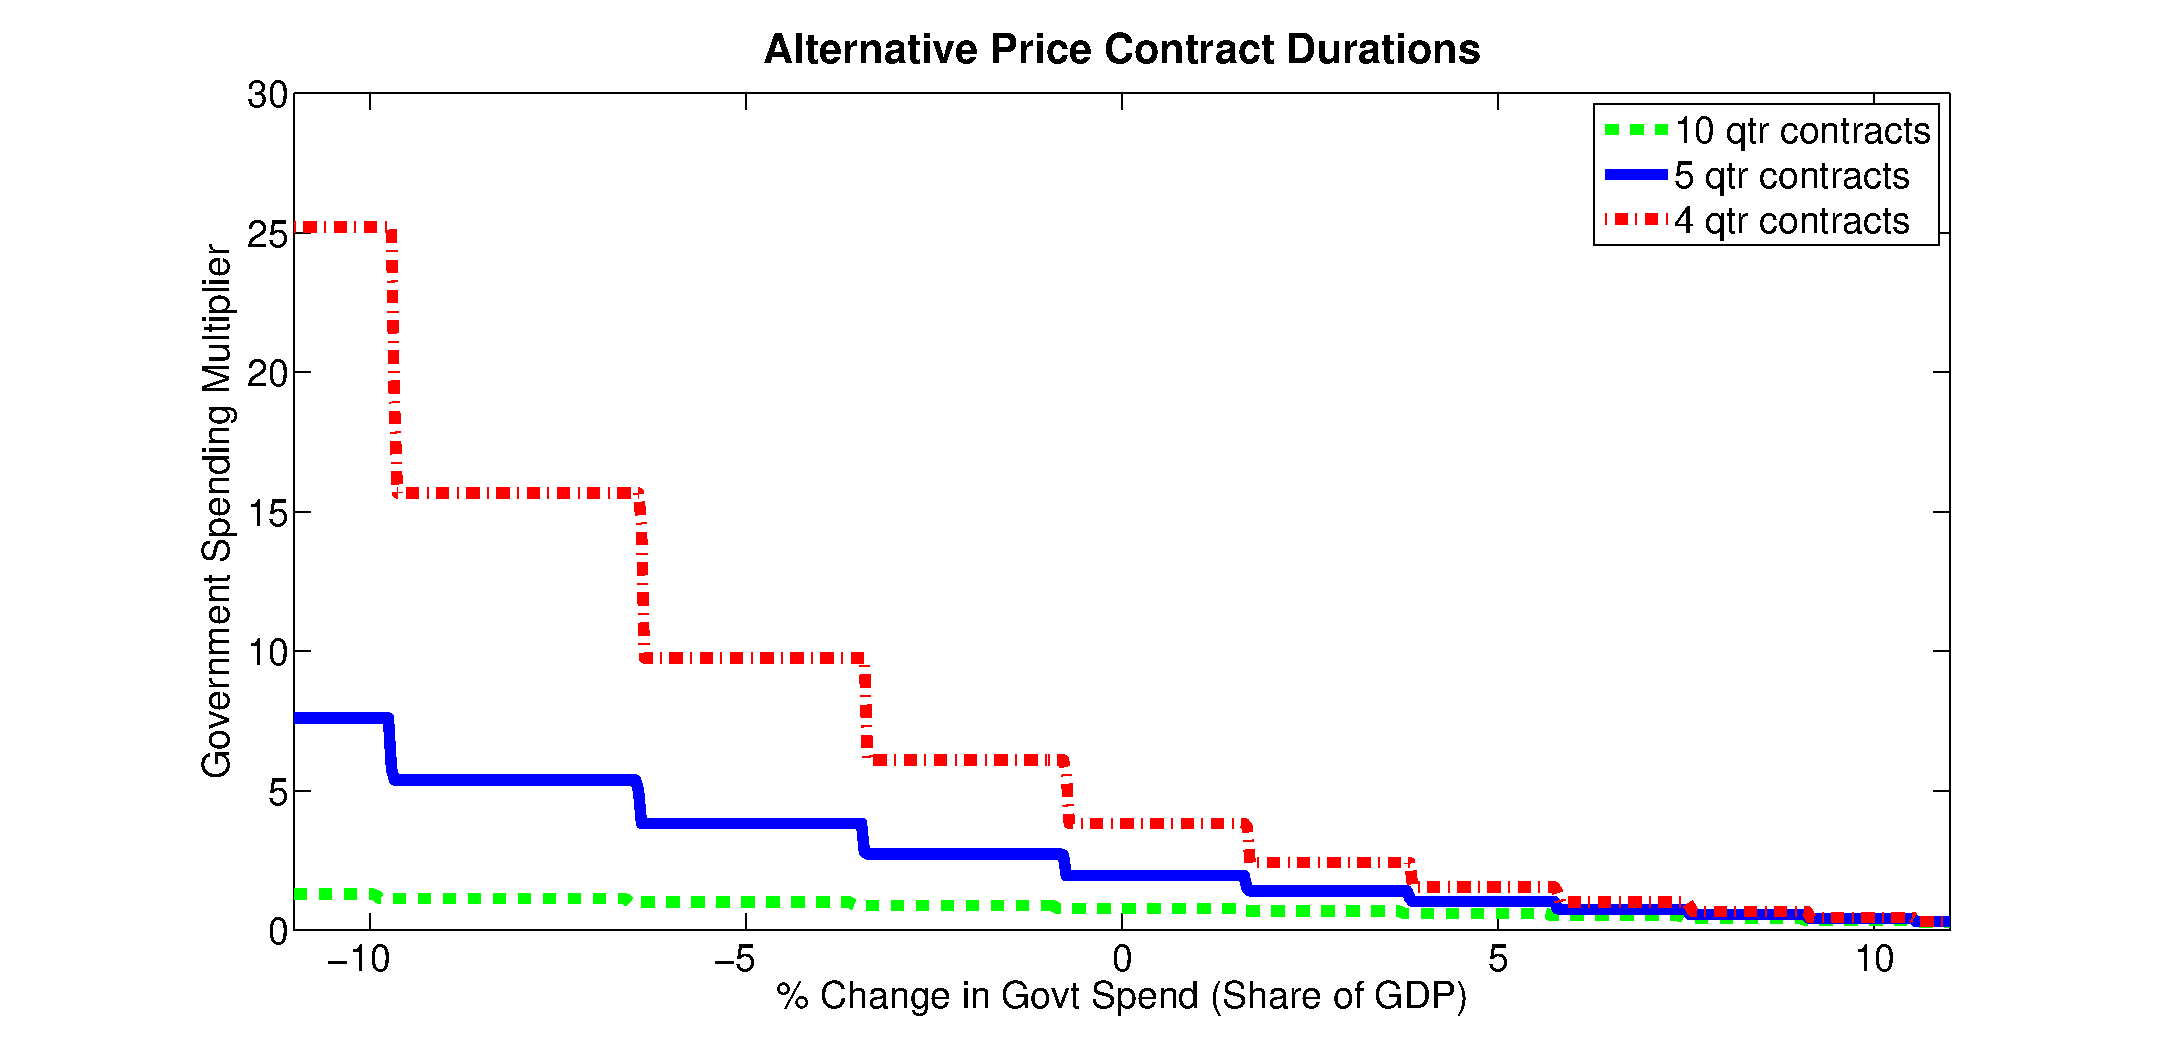
\includegraphics[width=0.8\textwidth]{paper/figures/figure-3-gsm-alternative-price.eps}
\caption{Spending Multiplier under Alternative Contract Duration}
\label{fig:mulalt}
\end{figure}

A large multiplier makes a strong case for government intervention. Figure \ref{fig:mulalt} tells, however, also another story and a word of caution is necessary here. Although we have a higher multiplier the more flexible the prices are, the drop in the multiplier caused by the shortening of the liquidity trap is also stronger in this case. The multiplier falls sharply with the level of government spending when prices are not very sticky. This observation leads to the important distinction between average and marginal multiplier, which is central for the paper we are analyzing.


\subsection*{Marginal vs. Average Multiplier}

The multiplier itself is a marginal concept. It tells by how much GDP grows if government increases spending by one percent. More important for policy making, however, is what \citet{Erceg.2014} have called the \textit{average multiplier}. Governments, while intervening in an economy, never do so by increasing spending only by a little amount. Rather, in face of an economic slow down, they often introduce stimulus packages of many millions of euros. In such a scenario, the marginal interpretation offered by the multiplier may not be very useful, especially if the multiplier varies significantly with the level of government spending. In face of a given-sized spending hike, the average multiplier tells us by how much \textit{on average} each extra euro spent by the government contributed to the increase in GDP. For the policy maker, it is of greater interest to know the average impact of higher spending (average multiplier) than the impact of the first euro spent (marginal multiplier), especially when the increase is considerable and the multiplier varies a lot with the size of government spending. This is exactly the case with the model of \citet{Erceg.2014}. In rough lines, the marginal multiplier is certainly higher in a liquidity trap, but it decreases at a fast rate once the government intervenes and through increases in government spending, shortens the duration of the liquidity trap.


% The average multiplier does not zoom in on a specific point - say 3\% increase – and answers the question by how much would GDP increase if spending increases by a marginal amount. Given the nature of the model and the decreasing multiplier, it is well known that the first euro spent will boost the economy by a greater amount than the last one. The concept of average multiplier abstracts from these differences and tells us what on average was the effect of each euro of extra spending on output. In this sense, the average multiplier is between the marginal multiplier when the government stays inert and the marginal multiplier when government has already stepped in and spent money to boost the economy.


Thus, an important message from the model is the following: although it may seem attractive to increase government spending in a liquidity trap because of the higher marginal multiplier, the overall effect on the economy might not be as pronounced as one is led to believe by analyzing the snapshot of the marginal multiplier when the crisis hit. This is so because the marginal multiplier decreases rapidly as the duration of the liquidity trap becomes shorter. It turns out that the average multiplier, i.e. the average contribution of each extra euro spent to GDP, is usually not as large as the marginal multiplier when government spending is at its steady state levels.

\subsection*{How to Calculate the Multiplier}

It turns out that the multiplier cannot be calculated analytically in the model. For that reason, we used a numerical approach to determine the multiplier schedule. For that, we used the Dynare loop to simulate the model with 551 different values for the government shock. We started with the scenario in which government \textit{cuts} spending by 11\% of GDP and went through increasing the government shock each time by 0.2\% until we reached the situation in which government \textit{increases} spending also by 11\% of GDP.

We then calculated the marginal multiplier as following. For each shock $ i \in \{2,\cdots, 551\} $ we computed:
\begin{equation}
  m_i = \frac{1}{g_y} \frac{(y_i - y_{i-1})}{(g_i - g_{i-1})} \nonumber \vspace{0.3cm}
\end{equation}
This ensured that the marginal interpretation of the multiplier is still valid, since the difference between $ g_i $ and $ g_{i-1}$ is very small. Also because of this small difference, we succeeded in plotting the multiplier schedule with the format of a stairway. Given that the distance between every two points in the graph is so small, the line linking values of multiplier values in two different liquidity traps appear to be perfectly vertical, even though strictly speaking this is not the case.

For the average multiplier we proceeded similarly. We found the government shock that roughly corresponds to the case in which there is no change in government spending or, in other words, the shock closest to zero. This shock turned out to be the 275th iteration of the loop. From that point we computed for each $ i \in \{276,\cdots, 551\} $:
\begin{equation}
  m^{avg}_i = \frac{1}{g_y} \frac{(y_i - y_{275})}{(g_i - g_{275})}. \nonumber
\end{equation}



\section{Fiscal Free Lunch}

We have seen that in the case where prices are more flexible, the multiplier can become very large with each extra euro spent by government boosting GDP by almost 4\%. Given that the multiplier is so high, would it be the case of a fiscal free lunch? A fiscal free lunch would occur if the extra economic activity generated by the fiscal stimulus is so high that the taxes collected over it are greater than the stimulus itself. Contrary to common-sense, an increase in spending would in fact reduce overall public debt compared to the case in which government does not intervene.

\begin{figure}[!th]
\centering
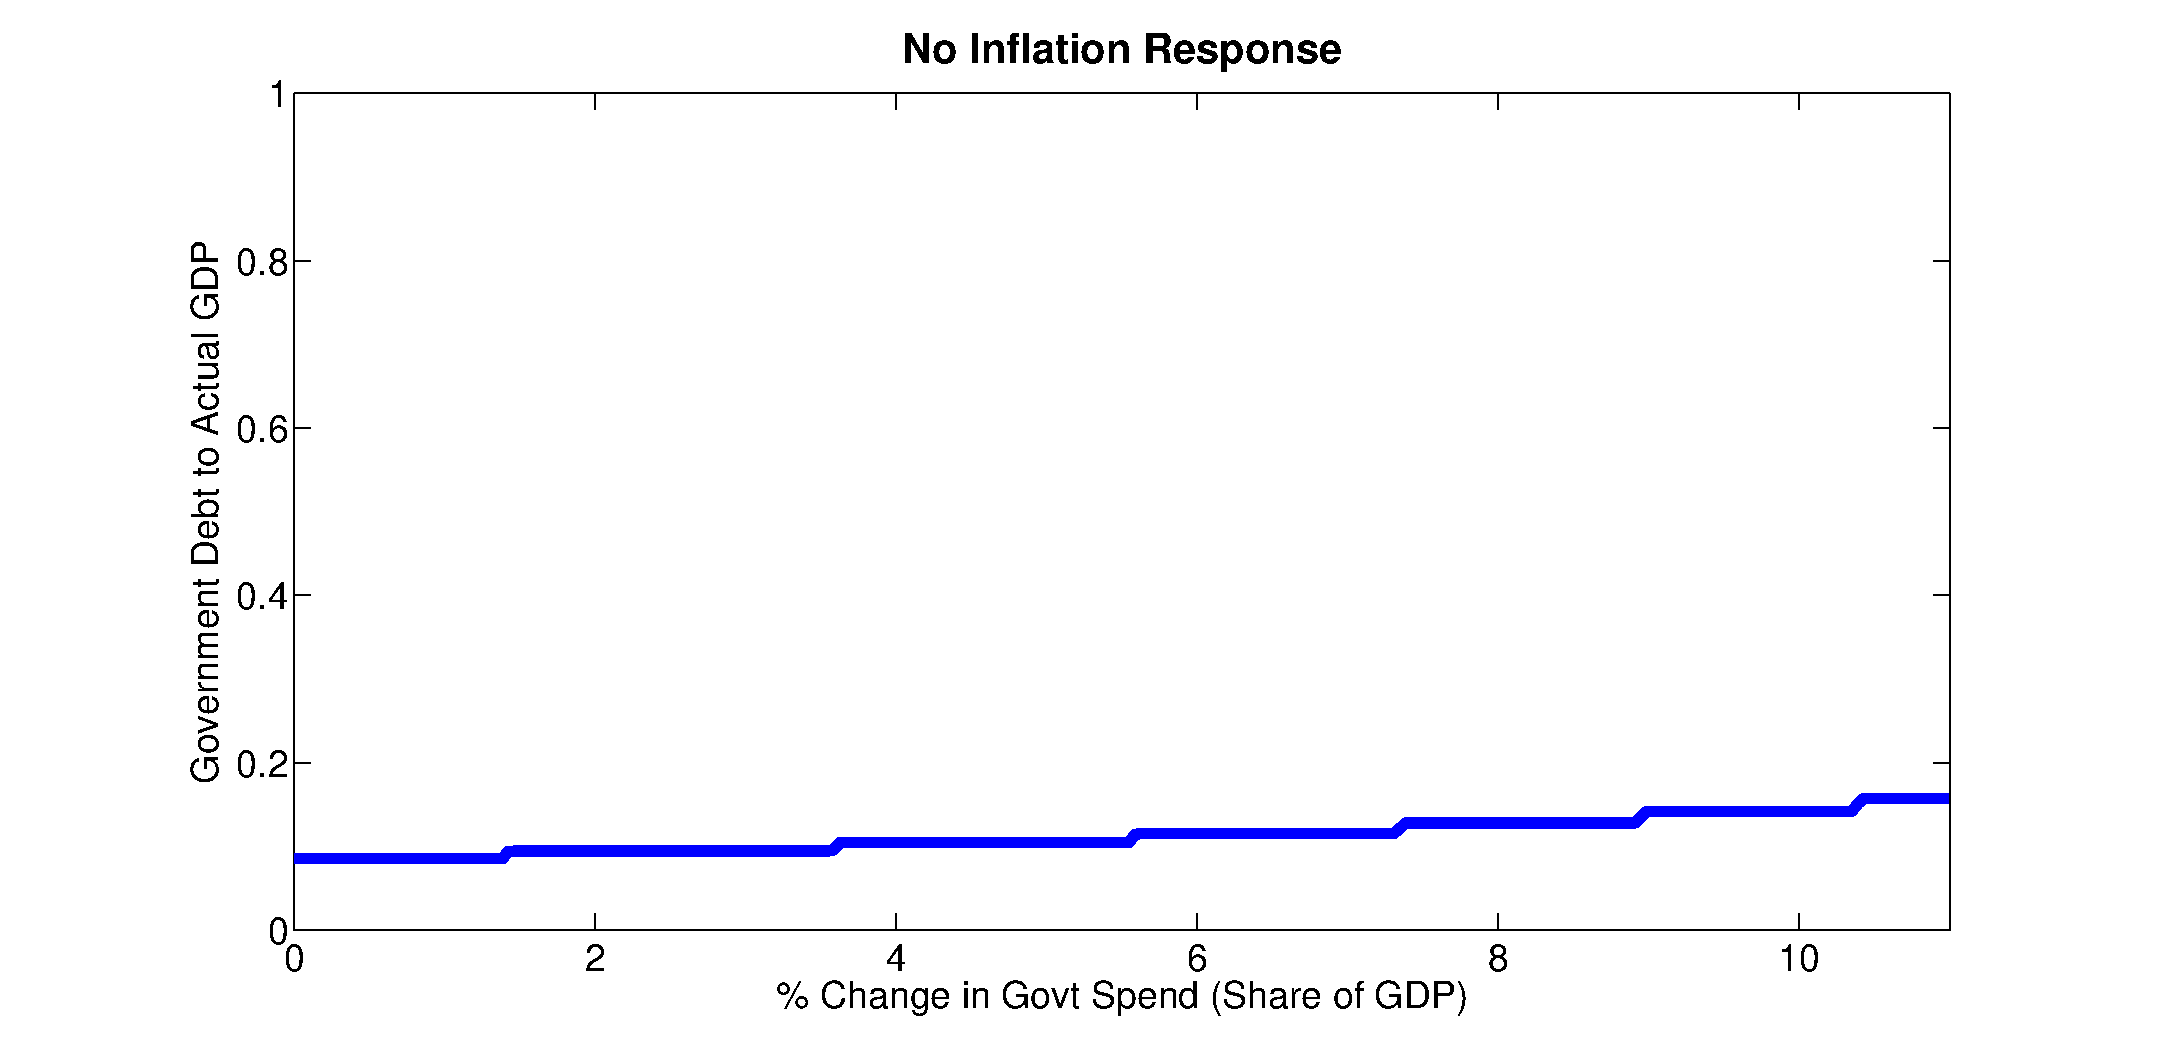
\includegraphics[width=0.8\textwidth]{paper/figures/figure-3-government-debt-no-inflation.eps}
\caption{Government Debt Response with No Inflation}
\label{fig:debtnoinflation}
\end{figure}

This question is best answered by analyzing Figure~\ref{fig:debt}. It depicts the marginal effect that government spending has on government debt. The striking conclusion of the model is that for four-quarter contracts, a spending hike of one percent of GDP causes the debt to fall by roughly 0.7 percentage points. In this very scenario, even increases in spending in amounts greater than 7\% of GDP would not only be self-financing but it would in fact decrease government debt. The fiscal free lunch is also observed for five-quarter contracts although not as pronounced as in the previous case. For more sticky prices (average contract duration of ten quarters and with no inflation in Figure~\ref{fig:debtnoinflation}), there is no fall in debt but still in this case the government stimulus comes at moderate budgetary costs. The rate at which debt increases with government spending is not so high.

\begin{figure}[!th]
\centering
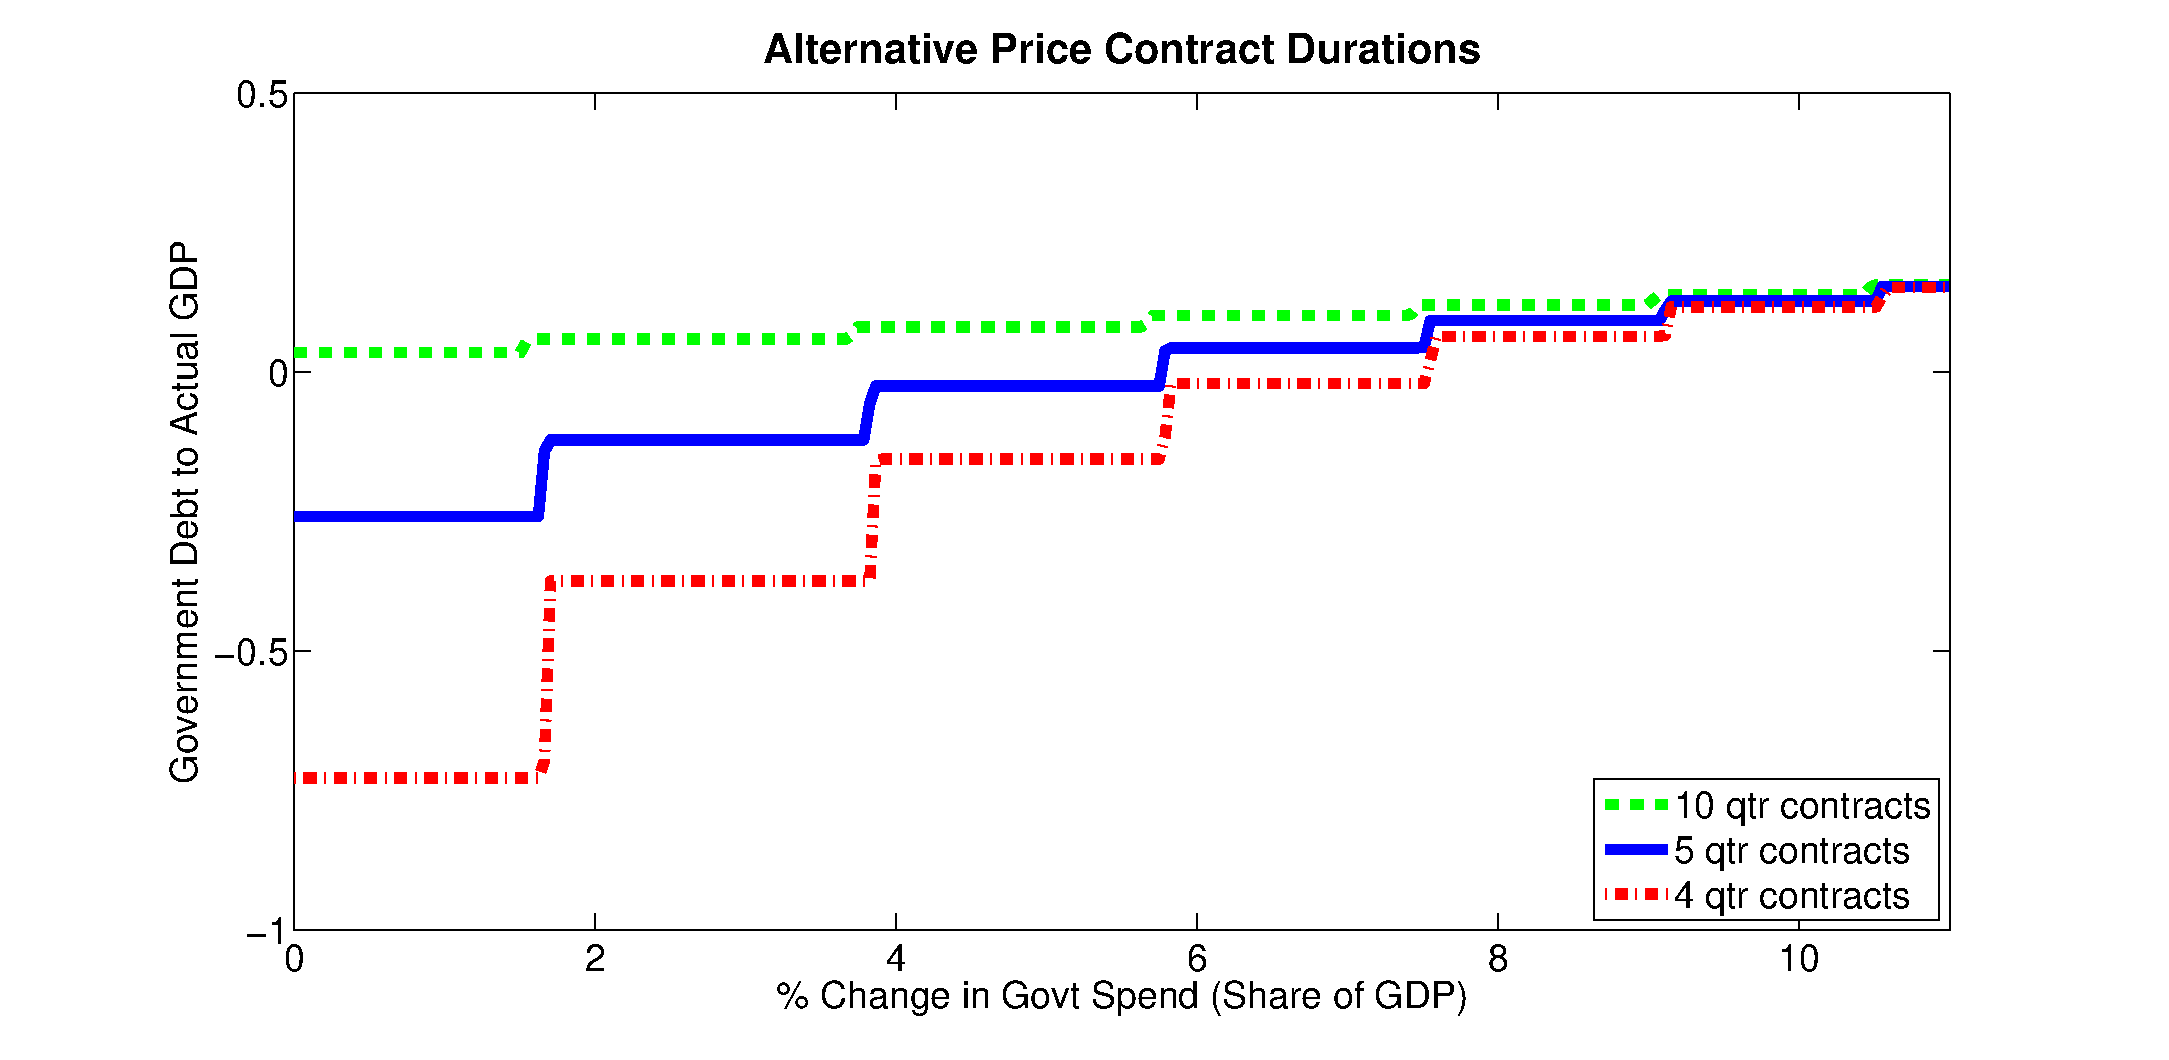
\includegraphics[width=0.8\textwidth]{paper/figures/figure-3-government-debt-alternative-prices.eps}
\caption{Government Debt Response under Alternative Contract Duration}
\label{fig:debt}
\end{figure}

The existence of a fiscal free lunch has an important flipside. If it is true that government can stimulate the economy at low or no costs while in a liquidity trap, it is also true – and maybe even more important to notice – that austerity measures in such a scenario can have very detrimental effects to the economy. A high multiplier means not only that increases in spending boosts GDP but also that cuts in spending when the economy is already depressed will deepen the recession even further.
